%***************************************************************************************
\section{Prior Uncertainty Propagation of the FEBA Tests}\label{app:tbl_results_uq_feba}
%***************************************************************************************

%----------------------------------------------------------------------------
\subsection{Clad Temperature Output ($TC$)}\label{app:tbl_results_uq_feba_tc}
%----------------------------------------------------------------------------

% FEBA Test No. 214 Prior Uncertainty Propagation, TC
\rotatebox{90}{\begin{minipage}{0.85\textheight}
    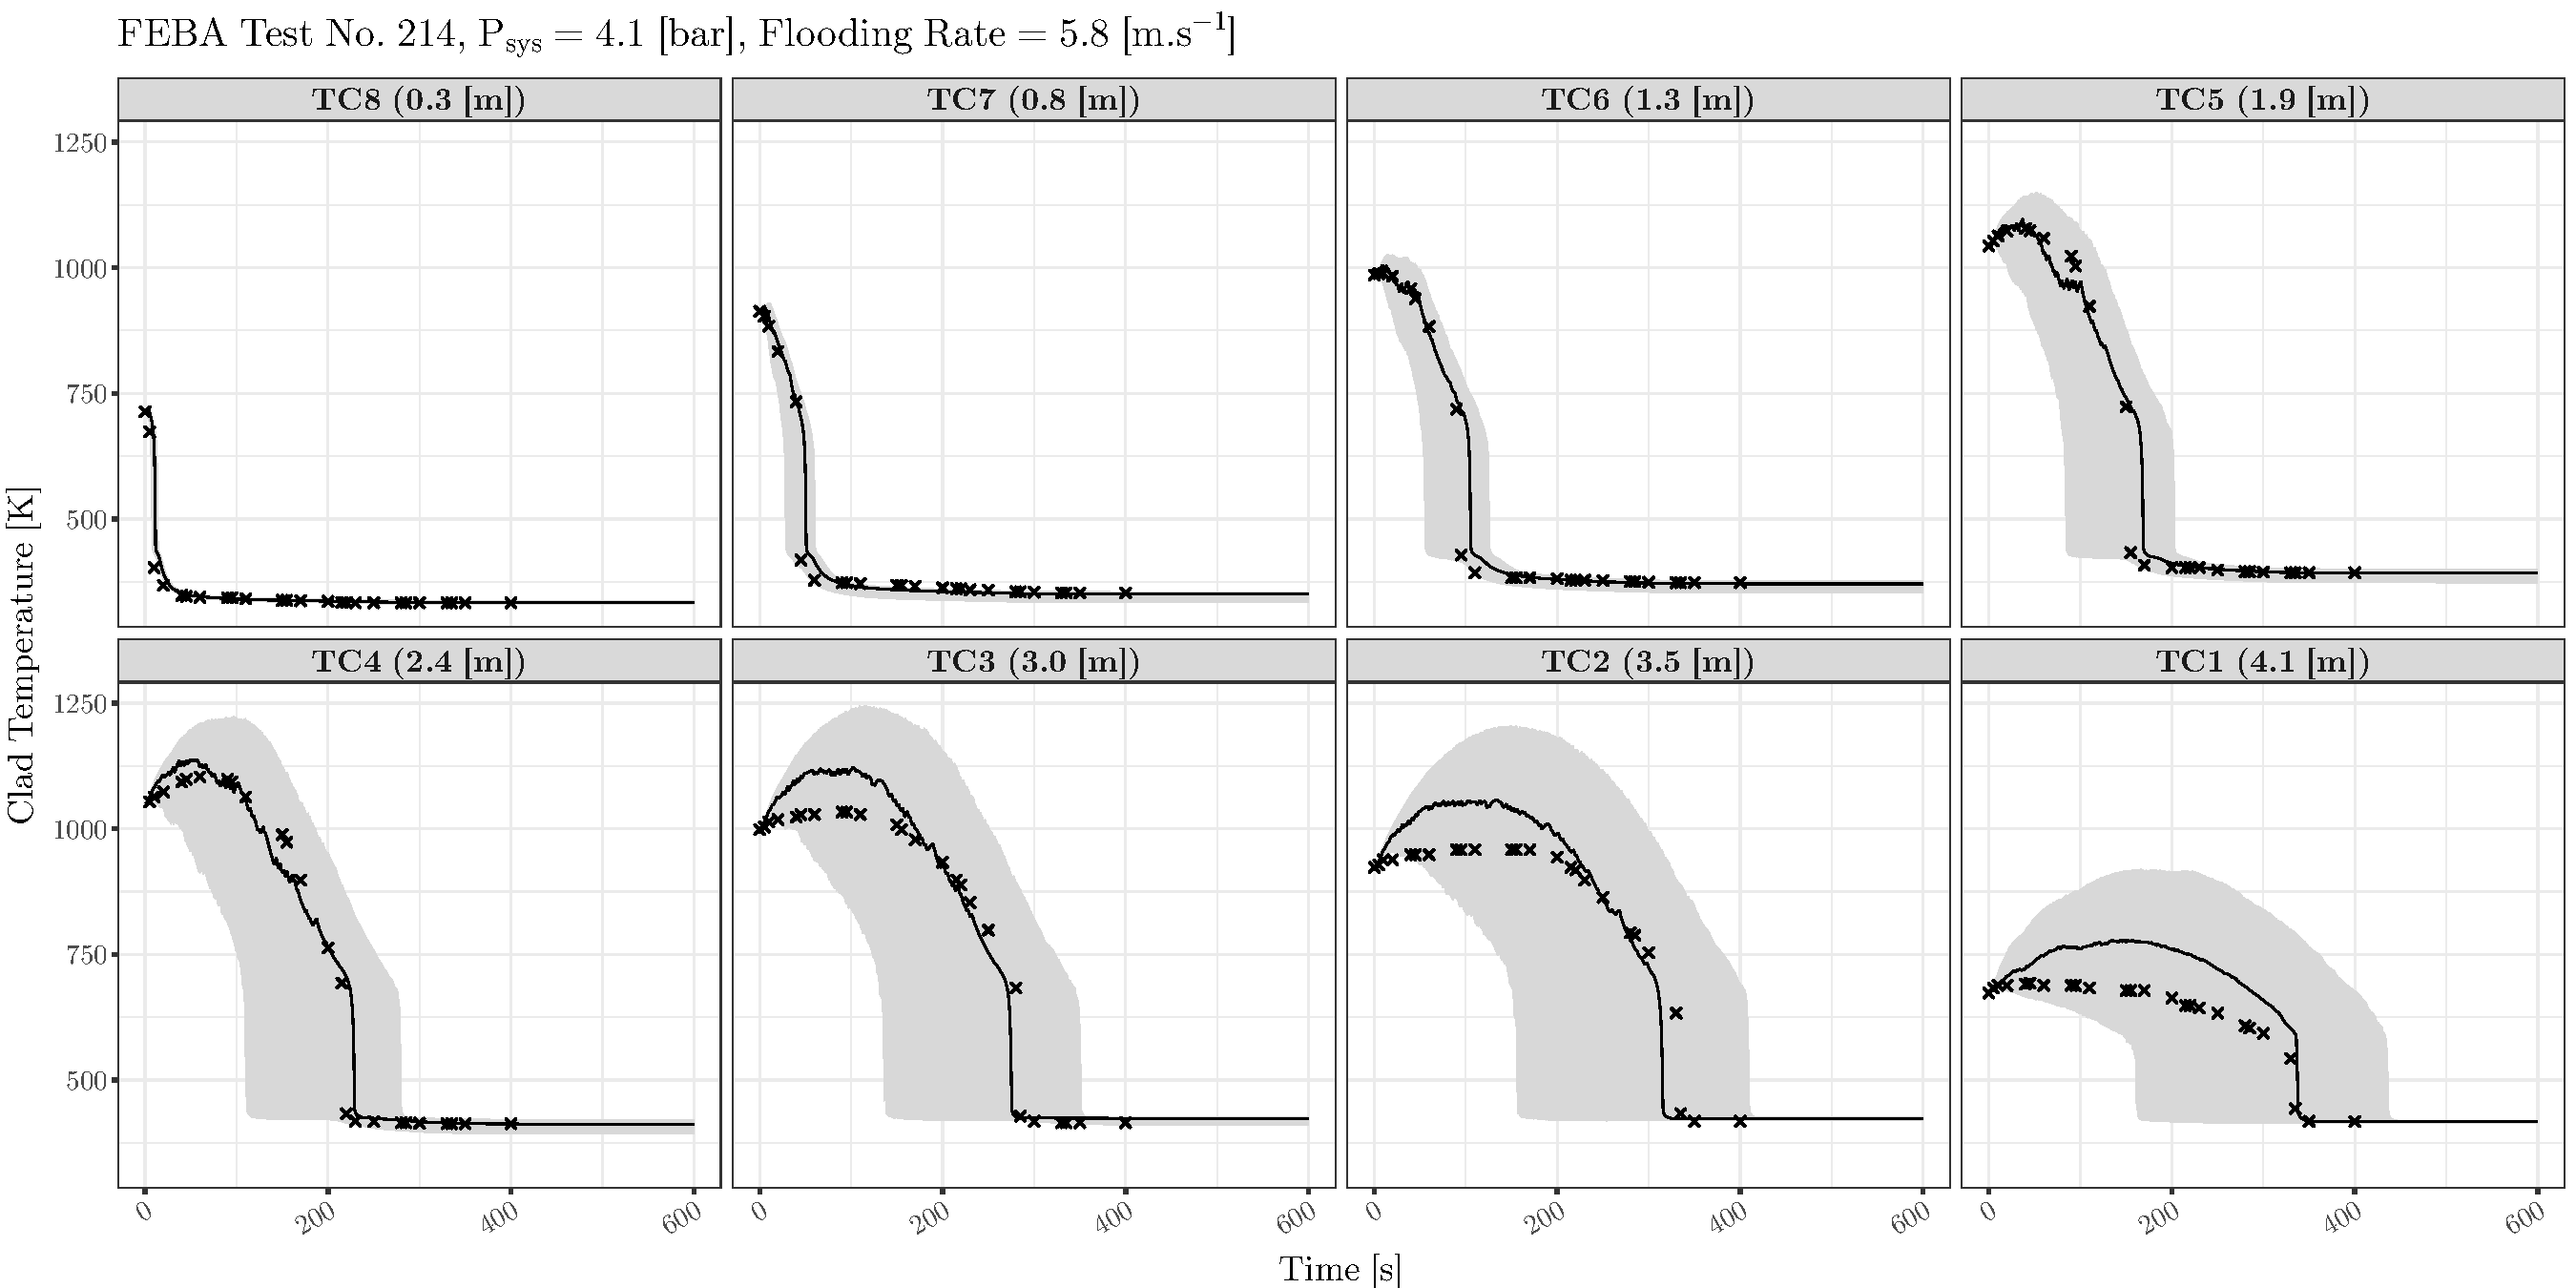
\includegraphics[width=1\textwidth]{../figures/chapter2/figures/plotTraceUQPriorTC214}
		\captionof{figure}[Prior uncertainty propagation for FEBA Test No. $214$ for cladding temperature output ($TC$).]{Uncertainty propagation of the prior parameters uncertainty for \gls[hyper=false]{feba} Test No. $214$ for cladding temperature output ($TC$) at different axial locations using \gls[hyper=false]{trace}. The uncertainty bound refers to the symmetric ($95\%$) probability, solid lines indicate the best-estimate simulation, and crosses indicate the experimental data.}
    \label{fig:ch2_plot_trace_uq_prior_tc_214}
\end{minipage}}
 
%-------------------------------------------------------------------------
\subsection{Pressure Drop Output ($DP$)}\label{app:tbl_results_uq_feba_dp}
%-------------------------------------------------------------------------

%----------------------------------------------------------------------------
\subsection{Liquid carryover Output ($CO$)}\label{app:tbl_results_uq_feba_co}
%----------------------------------------------------------------------------

% PC GP Metamodel Construction, Liquid Carryover output
%\clearpage
%\begin{sidewaysfigure}
%	\centering
%	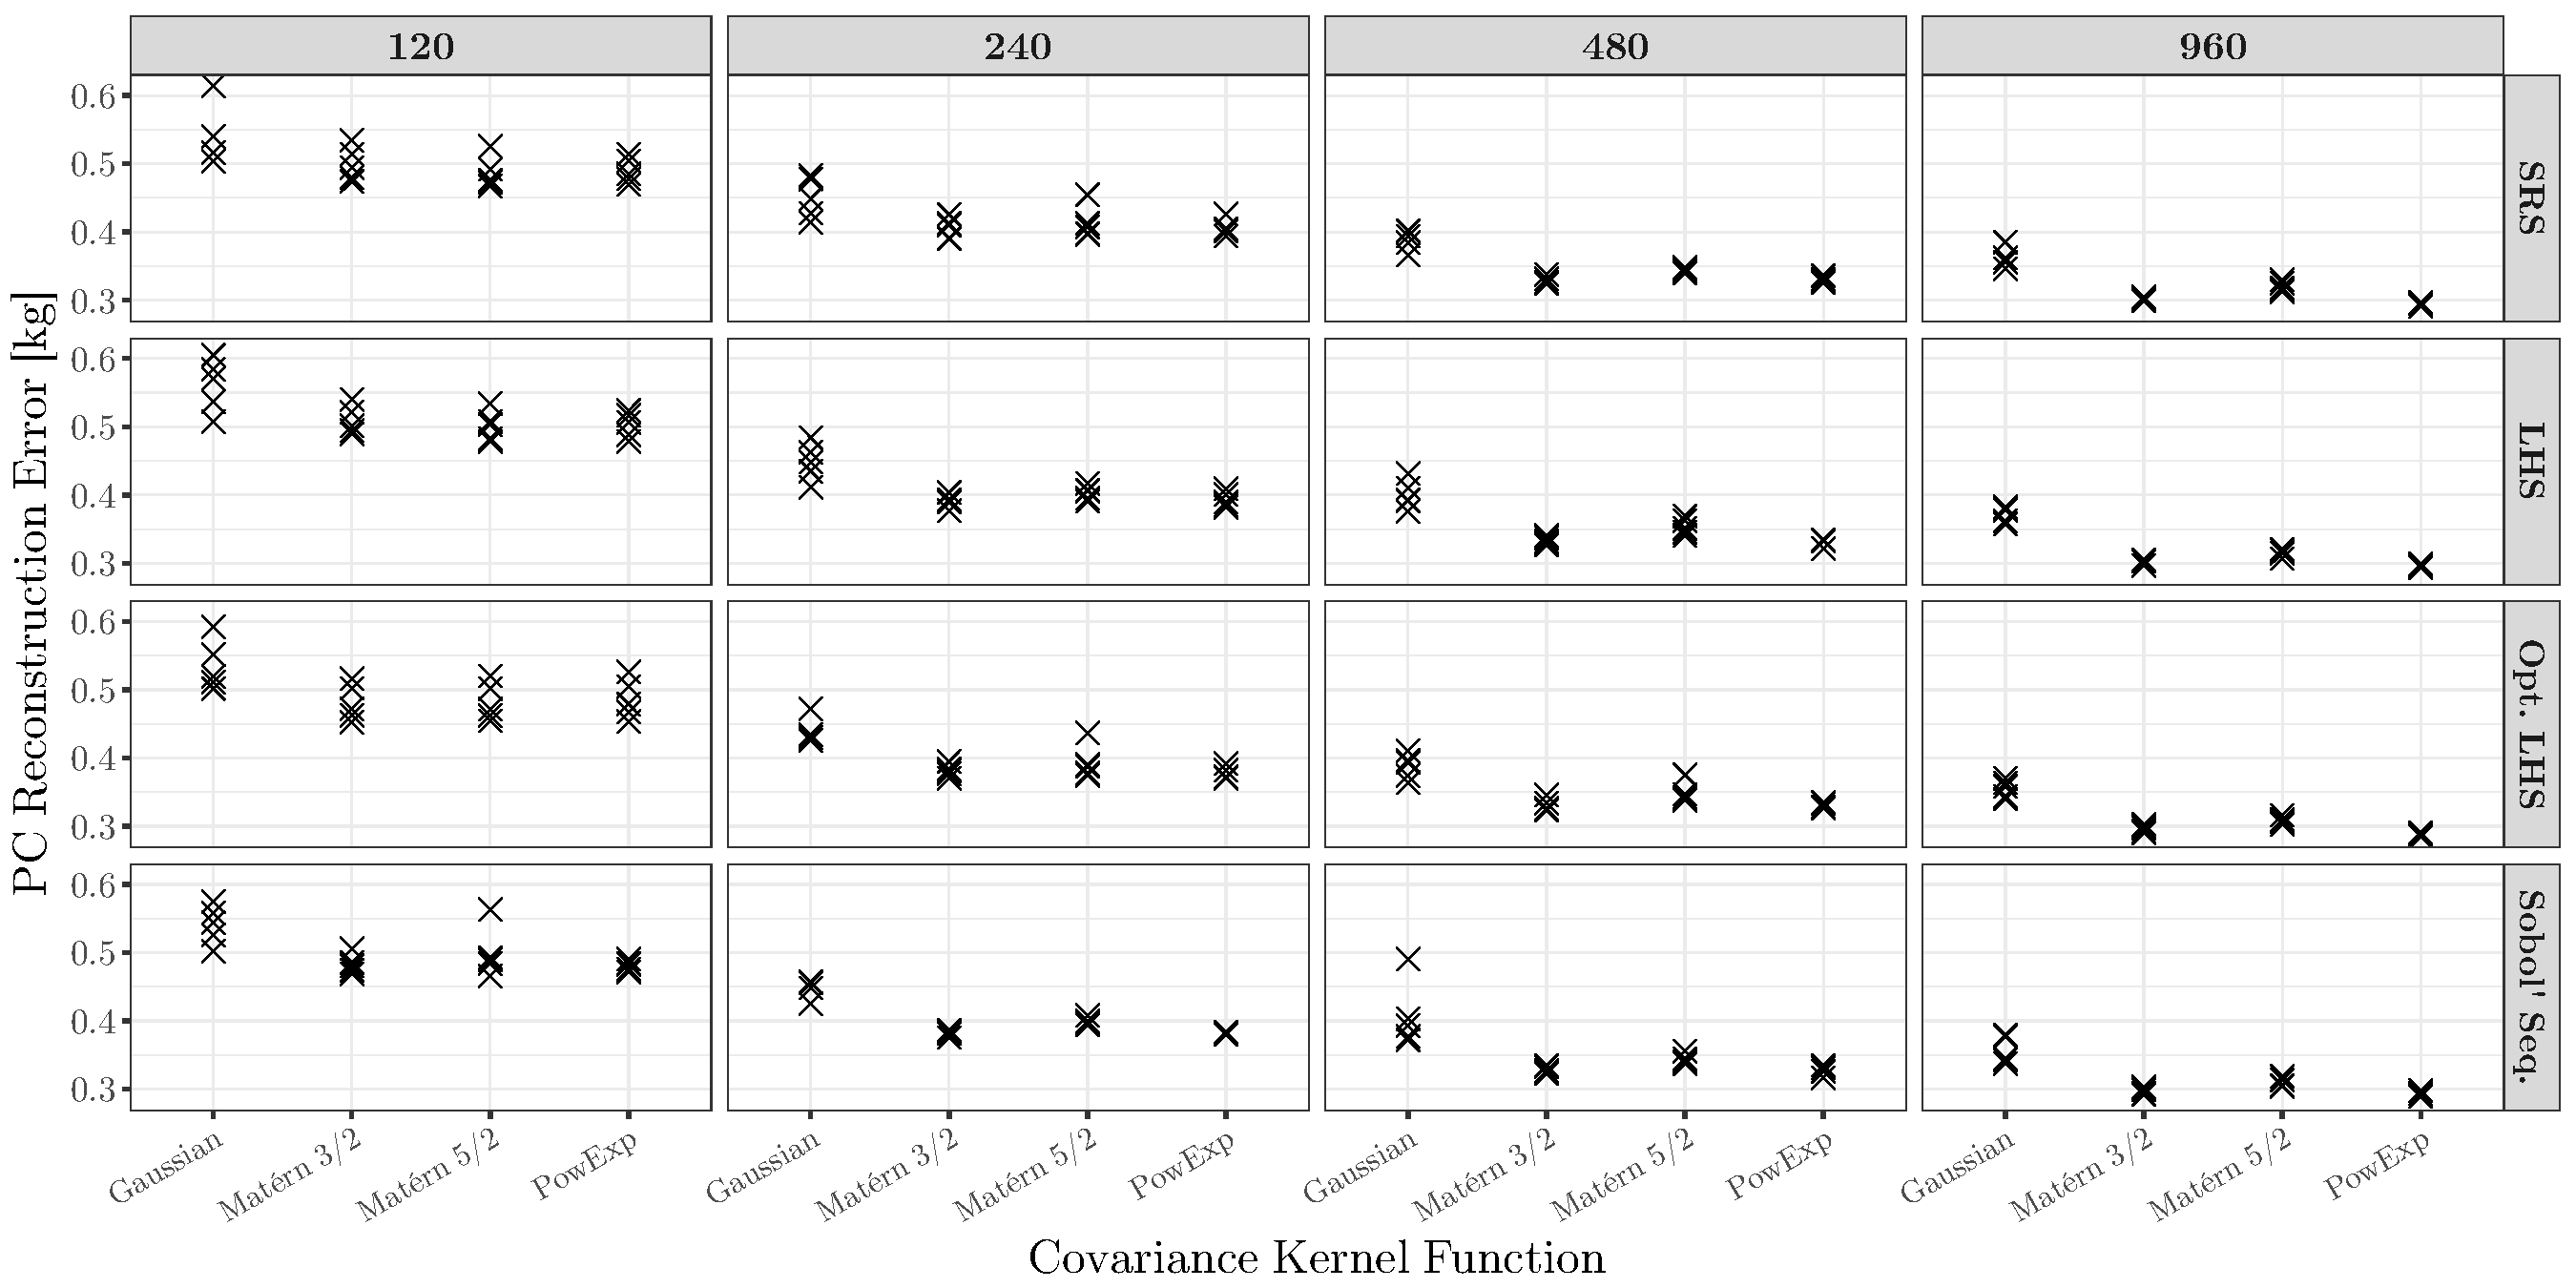
\includegraphics[width=1.0\textwidth]{../figures/chapter4/figures/plotPCGPConstructionCO}
%	\caption[The effect of training sample size, experimental design, and covariance function on the predictive performance of GP PC metamodel with respect to the liquid carryover output]{The effect of training sample size, experimental design, and covariance function on the predictive performance (in terms of \gls[hyper=false]{rmse}) of \gls[hyper=false]{gp} \gls[hyper=false]{pc} metamodel with respect to the liquid carryover output. $5$ \glspl[hyper=false]{pc} were used for the reconstruction.}
%	\label{fig:ch4_plot_pc_gp_construction_co}
%\end{sidewaysfigure}
\clearpage